
\part*{Impuls}


\section*{Luftwiderstand}


\subsection*{Vertikaler Fall}

Der Luftwiderstand ist proportional zum Quadrat der Schnelligkeit
und der Geschwindigkeit entgegengesetzt:
\begin{verse}
$\vec{F}_{w}=-c_{w}\cdot\frac{\rho A}{2}\cdot|\vec{v}|^{2}\cdot\vec{n}_{v}$

$c_{w}=$Widerstandszahl

\emph{$\rho=$}Luftdichte\emph{ $(1.293kg/m^{3})$}

$A=$Querschnittsfläche $\bot$ zu $\vec{v}$

$\vec{n}_{v}=\frac{\vec{v}}{|\vec{v}|}$
\end{verse}
Die Widerstandszahl $c_{w}$ hängt von der Geometrie des betrachteten
Körpers ab.


\subsection*{Maximale Fallgeschwindigkeit}
\begin{verse}
$m_{s}\vec{a}=\vec{F}_{g}+\vec{F}_{w}$

$m\dot{v}_{z}=-mg+c_{w}\cdot\frac{\rho_{Luft}A}{2}\cdot v_{z}^{2}$

$\Rightarrow\underset{t\rightarrow\infty}{lim\: v_{z}(t)}=\sqrt{\frac{g}{\gamma}}=\sqrt{\frac{2mg}{c_{w}\rho_{Luft}A}}$

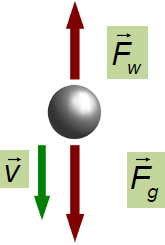
\includegraphics[scale=0.6]{Impuls/Fallgeschwindigkeit}
\end{verse}

\subsection*{Fallgeschwindgkeit Allgemein}

Geschwindigkeit als Funktion der Zeit:
\begin{verse}
$m\frac{d^{2}x}{dt^{2}}=mg-kv^{2}$

$v=\frac{dx}{dt}$

$\frac{dv}{dt}=g-\frac{k}{m}v^{2}$
\end{verse}

\subsection*{Ballistische Kurven}

Generell geht es darum, die Bahn eines Geschosses vorherzusagen.
\begin{verse}
$m\frac{d\vec{v}}{dt}=\vec{F}_{G}-k\cdot|\vec{v}|^{2}\cdot\vec{n}_{v}$

$\vec{n}_{v}=\frac{\vec{v}}{|\vec{v}|}$

$k=$Konstante $\left[\frac{kg}{m}\right]$
\end{verse}
Dieses Problem kann nur numerisch, in Koordinatenform angegangen werden:
\begin{verse}
$\left(\begin{array}{c}
\dot{v}_{x}\\
\dot{v}_{y}\\
\dot{v}_{z}
\end{array}\right)=\left(\begin{array}{c}
0\\
0\\
-g
\end{array}\right)-k\cdot\sqrt{v_{x}^{2}+v_{y}^{2}+v_{z}^{2}}\cdot\left(\begin{array}{c}
v_{x}\\
v_{y}\\
v_{z}
\end{array}\right)$

$\dot{v}_{x}=-kv_{x}\sqrt{v_{x}^{2}+v_{y}^{2}+v_{z}^{2}}$

$\dot{v}_{y}=-kv_{y}\sqrt{v_{x}^{2}+v_{y}^{2}+v_{z}^{2}}$

$\dot{v}_{z}=-g-kv_{z}\sqrt{v_{x}^{2}+v_{y}^{2}+v_{z}^{2}}$
\end{verse}

\section*{Impuls}


\subsection*{Definition}

Gegeben ist eine punktförmige Masse m mit einer Geschwindigkeit $\vec{v}$.\\
Der Impuls dieser Masse ist definiert als:
\begin{verse}
$\vec{p}=m\vec{v}$
\end{verse}
Der Impuls ist also ein Vektor.


\subsection*{Impuls einer ausgedehnten Masse}
\begin{verse}
$\vec{p}=\underset{Volume}{\int}\rho(\vec{r})\vec{v}(\vec{r})dV$

$\rho(\vec{r})=$Dichte am Punkt $\vec{r}$

$v(\vec{r})=$Geschwindigkeit am Punkt $\vec{r}$
\end{verse}
dm(r) ist ein Stücklein Masse. Die Gesamtmasse ist aus vielen Massenstücklein
zusammengesetzt, das Integral ist eine Summe über ganz kleine Stücklein:
\begin{verse}
$dm(\vec{r})=\rho(\vec{r})dV$
\end{verse}

\subsection*{Zusammenhang Impuls und Kraft}

Es gilt:
\begin{verse}
$\vec{F}=m\vec{a}$, $\vec{p}=m\vec{v}$
\end{verse}
Weiter können wir sagen:
\begin{verse}
$\frac{d\vec{p}}{dt}=\frac{d}{dt}(m\vec{v})=\frac{dm}{dt}\vec{v}+m\frac{d\vec{v}}{dt}$ 
\end{verse}
Falls die Masse zeitlich konstant ist $(\frac{dm}{dt}=0)$ gilt:
\begin{verse}
$\frac{d\vec{p}}{dt}=m\frac{d\vec{v}}{dt}=m\vec{a}=\vec{F}$

$\Rightarrow\frac{d\vec{p}}{dt}=\vec{F}$
\end{verse}
Die zeitliche Ableitung des Impulses eines Massenpunktes ist gleich
der Kraft, die auf ihn wirkt!


\section*{Impulserhaltung}

Für ein System miteinander wechselwirkender Massen aber ohne äussere
Kräfte ist der Gesamtimpuls eine Konstante.
\begin{verse}
$\vec{p}_{tot}=\underset{i}{\sum}m_{i}\vec{v}_{i}=const.$

$\frac{d\vec{p}_{tot}}{dt}=\frac{d}{dt}\left(\underset{i}{\sum}m_{i}\vec{v}_{i}\right)=\underset{i}{\sum}m_{i}\vec{a}_{i}=\underset{i}{\sum}\underset{j\neq i}{\sum}\vec{F}_{ij}^{intern}$
\end{verse}

\section*{Masseschwerpunkt}


\subsection*{Definition}
\begin{verse}
$\vec{r}_{CM}=\frac{\underset{i}{\sum m_{i}\vec{r}_{i}}}{\underset{i}{\sum}m_{i}}$
\end{verse}

\subsection*{Schwerpunktgeschwindigkeit}
\begin{verse}
$\vec{v}_{CM}=\frac{\vec{p}_{tot}}{\underset{i}{\sum}m_{i}}$
\end{verse}

\subsection*{Schwerpunktbeschleunigung}
\begin{verse}
$\vec{a}_{CM}=\frac{\underset{i}{\sum}m_{i}\vec{a}_{i}}{\underset{i}{\sum}m_{i}}$
\end{verse}

\section*{Schwerpunktsatz}

Die Änderungsrate des Impulses der im Schwerpunkt konzentrierten Gesamtmasse
der Teilchen ist gleich der Summe aller externen Kräfte.
\begin{verse}
$M_{tot}=\underset{i}{\sum}m_{i}$

$\vec{a}_{CM}=\frac{\overset{N}{\underset{i}{\sum}}\overset{K}{\underset{k}{\sum}\vec{F}_{ik}^{extern}}}{\underset{i}{\sum}m_{i}}\Longleftrightarrow M_{tot}\vec{a}_{CM}=\frac{d\vec{p}_{CM}}{dt}=\overset{N}{\underset{i}{\sum}}\overset{N}{\underset{k}{\sum}}\vec{F}_{ik}^{extern}$
\end{verse}
Eine Masse m übt gravitative Kräfte auf jeden Einzelteil einer Masse
M aus. Zwischen den Teilen von M wirken Kräfte, die M zusammenhalten:
\begin{verse}
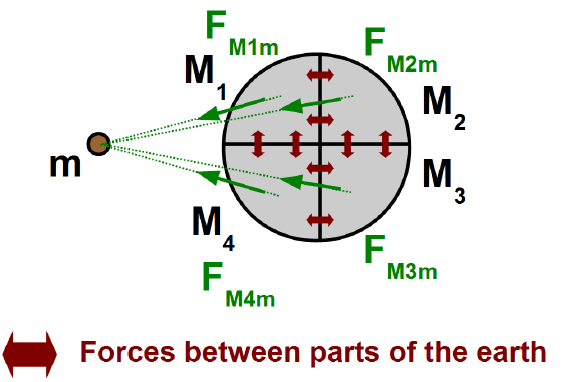
\includegraphics[scale=0.4]{Impuls/Schwerpunktsatz1}
\end{verse}
Aufgrund des Schewrpunktsatzes dürfen Sie so tun, als ob die von m
ausgeübte Kraft im Schwerpunkt von M auf ganz M wirken würde:
\begin{verse}
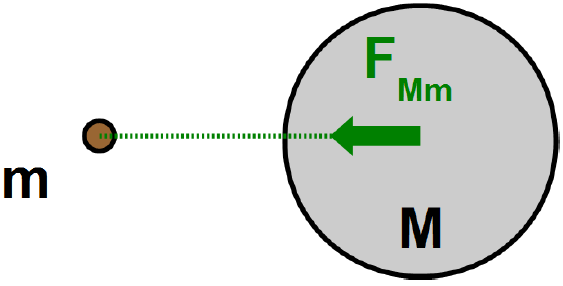
\includegraphics[scale=0.4]{Impuls/Schwerpunktsatz2}
\end{verse}
Wegen Newtons drittem Gesetz dürfen Sie jetzt schliessen, dass M eine
entsprechende Gegenkraft auf m ausübt:
\begin{verse}
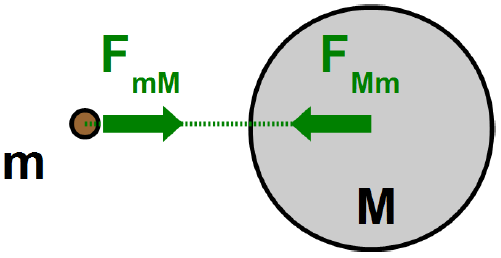
\includegraphics[scale=0.4]{Impuls/Schwerpunktsatz3}\end{verse}

